\chapter{Strutture Dati per Insiemi Disgiunti}
Le strutture dati per insiemi disgiunti sono utili alla rappresentazione efficace di famiglie dinamiche soggette a operazioni di:
\begin{itemize}
    \item \textbf{Make-Set(x)}: Introduzione di un singolo \{x\}.
    \item \textbf{Union(x,y)}: Unione degli insiemi disgiunti che contengono, rispettivamente, x e y.
    \item \textbf{Find-Set(x)}: Ricerca dell'insieme che contiene x.
\end{itemize}
Per l'analisi di queste strutture saranno prese in considerazioni $m$ operazioni di Make-Set, Union e Find-Set, comprendenti n operazioni di Make-Set. Varrà che $n\leq m$ e che il numero di union sia $\leq n-1$ dato che non le operazioni di union si fanno a due a due.
\section{Componenti Connesse in un Grafo}
Sia $G=(V, E)$ un grafo non orientato e siano $u \sim v$ per $u,v \in V$ se esiste un cammino da $u$ a $v$ in G. La relazione di $\sim$ è una relazione di equivalenza su $V$ e le \textbf{componenti connesse} di G sono le classi di equivalenza di $\sim$.
\begin{figure}[H]
    \centering
    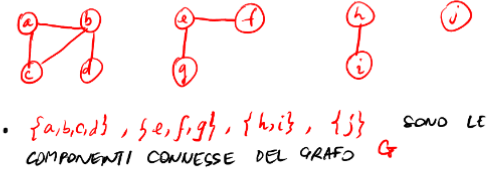
\includegraphics[width=0.5\linewidth]{Images/union_find/componenti_fortemente_connesse.png}
\end{figure}

\section{Generazione di Labirinti}
Allo stesso modo, possiamo anche generare dei labirinti sfruttando queste operazioni dato che, effettuando una serie di union, riusciremo a generare una sola componente connessa equivalente a un labirinto. 
\begin{figure}[H]
    \centering
    \begin{subfigure}{0.49\linewidth}
        \centering
        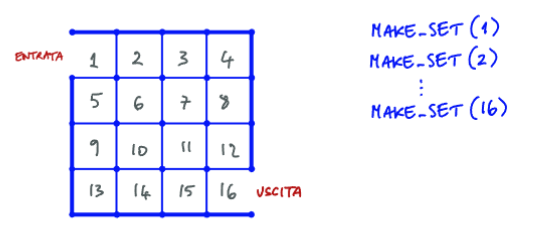
\includegraphics[width=\linewidth]{Images/union_find/labirinto_1.png}
    \end{subfigure}
    \hfill % Spazio flessibile
    \begin{subfigure}{0.49\linewidth}
        \centering
        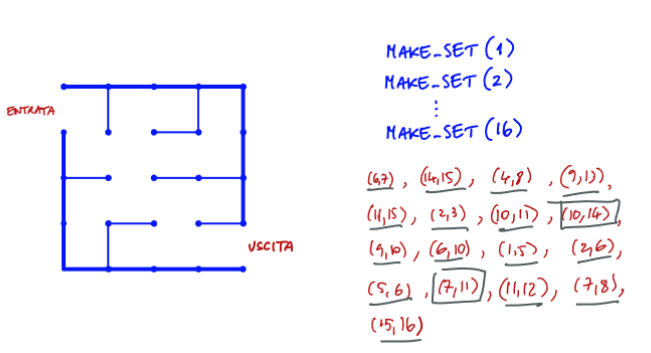
\includegraphics[width=\linewidth]{Images/union_find/labirinto_2.png}
    \end{subfigure}
\end{figure}

Per scegliere quali Union fare, si crea una lista di tutti i muri presenti e la si randomizza. Dopodiché scorri tutta la lista e, se i due elementi sono già nella stessa componente, non fai nulla, altrimenti li unisci tramite una union.
\section{Percolazione}
Un'altra interessante applicazione è la verifica della \textbf{percolazione} in un solido. Questa consiste nel passaggio lento di un liquido in uno specifico solido in considerazione. Immaginiamo questa situazione:
\begin{figure}[H]
    \centering
    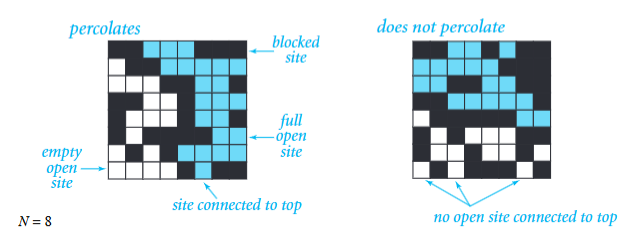
\includegraphics[width=0.5\linewidth]{Images/union_find/percolazione.png}
\end{figure}

Come possiamo vedere, a sinistra esiste un percorso dalla parte sopra alla parte sotto del blocco, per cui abbiamo percolazione; al contrario, nel blocco destro notiamo come l'acqua non possa passare a causa di blocchi non vuoti. Questo tipo di eventi può essere simulato in una griglia $N \times N$ per cui, ogni blocco, può essere pieno con probabilità $p$ e vuoto con probabilità $1-p$. Noteremo che, maggiore sarà $p$ e maggiore sarà la probabilità di percolazione.

\section{Implementazione di Insiemi Disgiunti}
Andiamo per gradi a vedere come poter implementare questo tipo di strutture dati. La scelta più banale ricade su una semplice lista di nodi, per cui:
\begin{figure}[H]
    \centering
    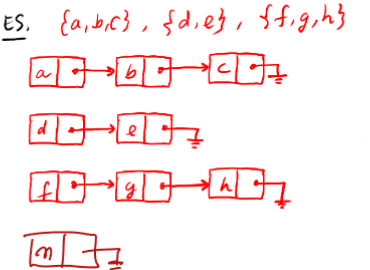
\includegraphics[width=0.4\linewidth]{Images/union_find/lista_semplice.png}
\end{figure}

Per quanto riguarda le operazioni vediamo che:
\begin{itemize}
    \item \textbf{Make-Set}: Ovvia, ci basta aggiungere sempre in testa.
    \item \textbf{Find-Set}: Possiamo utilizzare un riferimento alla Tail per capire a quale insieme si appartiene.
    \item \textbf{Union}: L'implementazione non è poi così semplice. 
\end{itemize}

Per ciò, decidiamo di modificare la nostra lista facendo sì che in ogni nodo vi sia un puntatore al \textbf{rappresentante} e uno al prossimo nodo nella lista.
\begin{figure}[H]
    \centering
    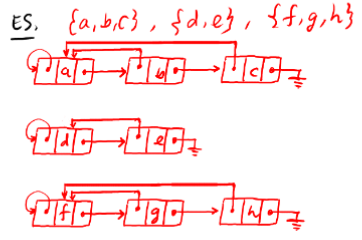
\includegraphics[width=0.4\linewidth]{Images/union_find/lista_2.png}
\end{figure}
In questo caso vediamo che:
\begin{itemize}
    \item \textbf{Make-Set}: Ovvia, come prima.
    \item \textbf{Find-Set}: Mediante il calcolo di $rapr[x]$ è immediato.
    \item \textbf{Union}: Effettuiamo una concatenazione e successivamente aggiorniamo tutti i campi rappresentante.
\end{itemize}

Ci rendiamo però conto come l'unione richieda necessariamente di scorrere tutta la lista per trovare la tail. Per evitare ciò, possiamo tenere un \textbf{nodo fittizio} all'inizio della lista che contiene le informazioni che riguardano la tail e la head per evitare di scorrere tutta la lista. 
\begin{figure}[H]
    \centering
    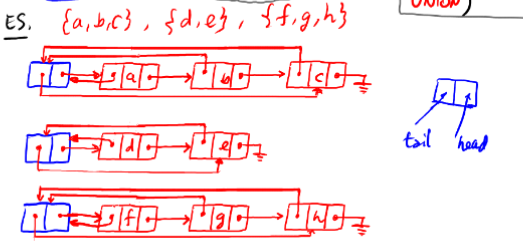
\includegraphics[width=0.7\linewidth]{Images/union_find/lista_3.png}
\end{figure}

Infine, al fine di ottimizzare ulteriormente il processo, possiamo anche eliminare il campo tail e fare tutte le unioni in testa dopo l'head.
\begin{figure}[H]
    \centering
    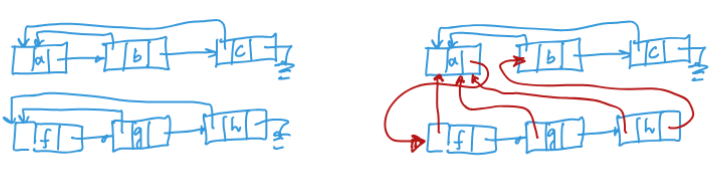
\includegraphics[width=0.7\linewidth]{Images/union_find/eliminazione_head.png}
\end{figure}

Consideriamo una sequenza di $2n-1$ operazioni e ragioniamo su queste:
\begin{figure}[H]
    \centering
    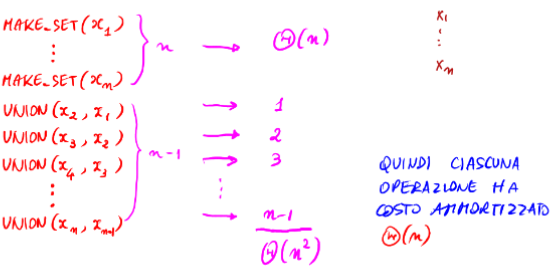
\includegraphics[width=0.8\linewidth]{Images/union_find/analisi_1_senza_euristica.png}
\end{figure}

I costi delle varie union derivano principalmente dall'aggiornamento del campo rappresentante delle varie liste che, come possiamo notare, sono sempre in ordine $union(x_i, x_{i-1})$. Questo è scelto per mostrare il caso peggiore poiché la lista più lunga è sempre $x_{i-1}$ ed è quella che, quindi, subirà tutti gli aggiornamenti. 
Da qui, intuitivamente, possiamo applicare un'euristica chiamata \textbf{Unione per Ranghi} in cui appendiamo la lista più corta a quella più lunga così da fare meno aggiornamenti possibili. Per fare ciò, tenendo ancora in considerazione il nodo fittizio, aggiungiamo anche il campo \textbf{size} che ci indica la lunghezza della lista che servirà proprio per fare il confronto durante l'unione.
Da qui, la seguente analisi:
\begin{figure}[H]
    \centering
    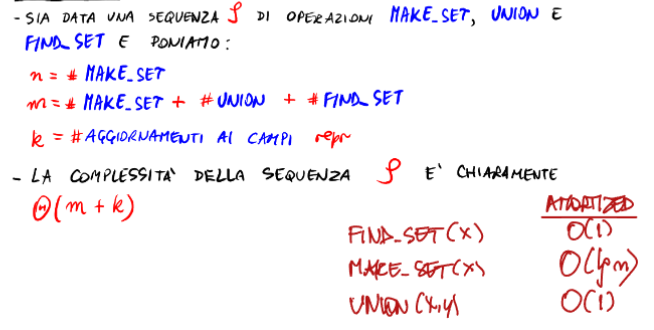
\includegraphics[width=0.9\linewidth]{Images/union_find/analisi_2_con_euristica.png}
\end{figure}

Questa analisi è fatta poiché, grazie all'euristica di unione per ranghi, ogni aggiornamento di rappresentante, la lista contenente x aumenta di almeno 2. Quindi il campo $rapr[x]$ può cambiare al più $\lfloor log(n)\rfloor$\footnote{Ciò deriva dal fatto che se x appartiene a una lista lunga n, possono esserci state al massimo $\lfloor log(n)\rfloor$ union, e quindi può aver cambiato un massimo di $\lfloor log(n)\rfloor$ rappresentanti.} volte. Di conseguenza, il numero totale di aggiornamenti del campo $rapr$ di tutti i nodi è $O(nlog(n))$, per cui, la complessità della sequenza è $O(m+n log(n))$.

\section{Insiemi Disgiunti mediante Alberi Disgiunti}
Un modo per migliorare ulteriormente l'implementazione è tramite l'utilizzo di alberi disgiunti con euristiche di \textbf{unione dei ranghi} e \textbf{compressione dei cammini}.
\begin{figure}[H]
    \centering
    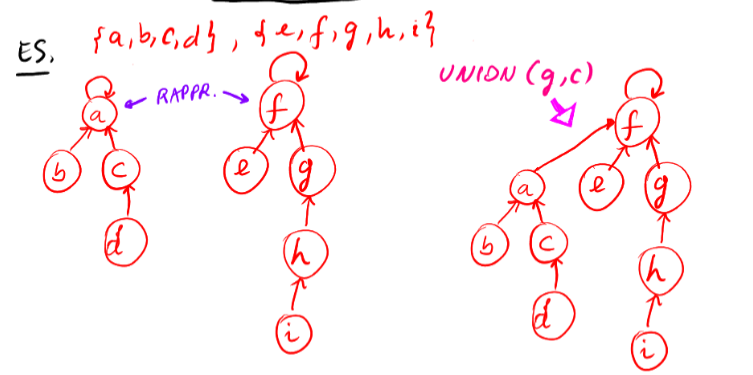
\includegraphics[width=0.7\linewidth]{Images/union_find/alberi_disgiunti.png}
\end{figure}
Definiamo in maniera opportuna il rango dell'albero legandolo al numero di archi del cammino semplice più lungo dal nodo x a una foglia. Anche in questo caso si sceglie di innestare il rango più piccolo in quello più alto e, nel caso di parità, si sceglie arbitrariamente.

L'euristica della compressione dei cammini consiste nell'ottimizzazione della find-set per iterazioni successive. Quindi, quello che facciamo è prendere tutti i nodi incontrati nell'esecuzione di una find-set e li innestiamo alla radice.
\begin{figure}[H]
    \centering
    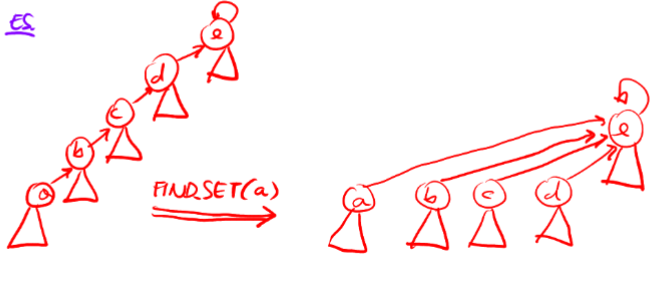
\includegraphics[width=0.7\linewidth]{Images/union_find/find_set_alberi.png}
\end{figure}
Per quanto riguarda le complessità utilizzando le euristiche vediamo:
\begin{figure}[H]
    \centering
    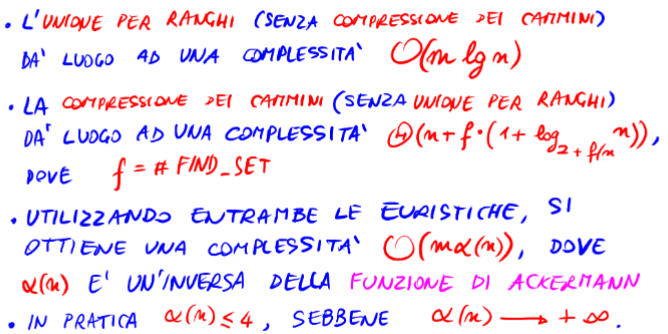
\includegraphics[width=0.7\linewidth]{Images/union_find/analisi_1_alberi.png}
\end{figure}